% !TEX root = Master.tex


So far we explored the data pinpointing multiple characteristics of article unit sales along with other features in an aggregate or grouped frame. This section will briefly highlight some additional aspects of demand quantities regarding individual articles and the associated limitations.
\\

Straight away, the biggest challenge is the life cycle of the articles. A sample of seven articles will list some these challenges. The course of those article sales is plotted in \autoref{fig:article_sample}. Article "5040" for example has only a lifespan of a 18 weeks and there are 12,679 out of 26,203 distinct articles having even less than that, which is almost half of the dataset. There are thousands of articles which have a lifespan of single digit (in weeks). This troublesome fact makes it very hard to apply any kind of promising quantitative methods. Nevertheless, this issue will be discussed in later parts of this paper. HERE SOME REFERENCE ON SECTION OR SUBSECTION TO BE WRITTEN!!!!
\\


\begin{figure}[H]
\centering
  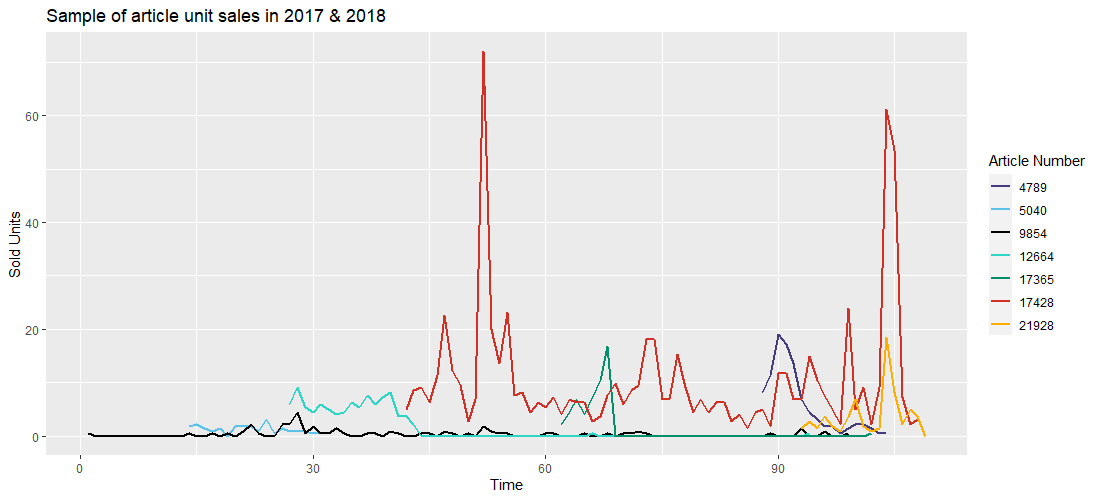
\includegraphics[width=0.95\linewidth]{figures/article_sample.png}
  \caption{Sample of seven articles and their demand quantity life cycles}
  \label{fig:article_sample}
\end{figure}



MAYBE (BETTER) WRITE SOME EXTRA CHALLENGES HERE ON INDIVIDUAL ARTICLES!!!!!



